% Appendix. It does not count toward the four pages. It carries what a replication needs and what the protocol
% promised to report: the rig's settings, the fixed analysis and stop rules, deviations, counts, and two side records.
% It also carries what the main text had no room for (method.tex lists it in its header), from protocol/protocol.md,
% draft 0.3: read that document beside this file when the protocol changes.
% Numbers: macros (generated/ and numbers_by_hand.tex), or typed with "% src:" on the line where they are known.

% ======================================================================================================================
\section{The rig's settings}
\label{app:rig}
Tables~\ref{tab:rig} and~\ref{tab:rigb} list the rig's settings in the categories of the workshop's checklist.
None of these settings was varied, so this study cannot determine how the tolerance radius depends on them.

\begin{table*}[t]
\caption{The rig's settings, in the categories of the workshop's Design Choice Reporting Checklist (continued in Table~\ref{tab:rigb}).}
\label{tab:rig}
\centering
\footnotesize
\begin{tabular}{@{}p{0.14\textwidth}p{0.17\textwidth}p{0.62\textwidth}@{}}
\toprule
Category & Setting & Value \\
\midrule
Hardware and embodiment & Arm & SO-101 follower and leader \cite{therobotstudio2026so100}; \rigArmBuild{} \\
 & Gripper & \rigGripper{} \\
 & Object and basket & Cube of \cubeEdge~mm: \rigCube. Basket: \rigTray{} \\
 & Workspace & Grid of $\gridCols\times\gridRows$ cells of \cellSize~mm, fixed to the table by two tags (\rigTags); light box: \rigLighting{} \\
Motors and actuation & Servos & Feetech STS3215; \rigServoVariant{} \\ % src: protocol/protocol.md, section 3 (the model); the variant is copied from the rig
Kinematics & Joints, calibration & Five arm joints and a gripper; \rigCalibration{} \\ % src: docs/reference/lerobot101-interfaces.md, section 1 (joint order)
Controller gains and rates & Servo position loop & \rigServoGains{} \\
 & Control rate & \execControlRate~Hz requested; \execControlRateAchieved~Hz achieved in policy trials \\
 & Limits on a command & Per-step clamp of \execClamp degrees; a policy's first command within \handoffTolerance degrees of the arm's pose on every joint, a replay's within \handoffToleranceReplay; stall rule: \rigStallRule{} \\
Action spaces & Action & \rigActionSpace{} \\
Observations & Cameras & Front: \rigFrontCamera, \rigCameraMount. Wrist: \rigWristCamera. Both \rigImageSize pixels at \rigCameraRate~Hz; \rigCameraSettings{} \\
 & Other inputs & \rigStateInput{} \\
\bottomrule
\end{tabular}
\end{table*}

\begin{table*}[t]
\caption{The rig's settings, continued: demonstrations, the policy, and the reset distributions.}
\label{tab:rigb}
\centering
\footnotesize
\begin{tabular}{@{}p{0.14\textwidth}p{0.17\textwidth}p{0.62\textwidth}@{}}
\toprule
Category & Setting & Value \\
\midrule
Demonstrations & Interface & Leader arm. Recording rate in Hz: \rigTeleopRate. Episode length in seconds: \rigEpisodeSeconds{} \\
 & Budget and layout & \nDemos per dataset. Clustered: \nDemosPerCell at each of \nPointsClustered points. Spread: \nPointsSpread positions, planned at least \spreadMinSpacing~mm apart (measured: at least \spreadSpacingMin~mm) \\
 & Recording & \nSittings recording sessions on one day, in the order clustered, spread, spread, clustered; practice before the first session was not recorded; \nRerecordedClustered clustered and \nRerecordedSpread spread episodes were recorded again. Recorded on the previous day and not used: 31 clustered episodes (Appendix~\ref{app:faults}) and 5 test episodes of the recorder \\ % src: data/recording/*_placements.jsonl (the sessions and their order; \nRecordingDays is 1); tolrad-clustered-v1-attempt1 (4 lines) and -attempt2 (27); tolrad-smoke2, 3 and 4 (1, 2 and 2 lines); docs/runbook/02-arm-and-recording.md, step 4 (practice, nothing recorded)
 & Start states & Set with the overlay, then measured from each episode's first frame: \demoPlacementErrorMedian~mm from the planned target at the median, \demoPlacementErrorMax~mm at most \\
 & Trained on & \nDemosTrainedClustered clustered and \nDemosTrainedSpread spread episodes; held out for an evaluation loss: \trainHeldOut{} \\
Policy (held fixed; not a checklist category) & Model and training & ACT \cite{zhao2023learning}, \trainParams~M parameters, \trainBackbone backbone, chunk of \trainChunk steps, batch \trainBatch, learning rate \trainLearningRate, seed \trainSeed, image augmentation \trainAugmentation; one run per dataset on \trainHardware, LeRobot \trainLerobotVersion; evaluated at step \evalCheckpoint{} \\
 & Execution & Temporal ensembling with coefficient \execEnsembleCoeff and inference at every step; attempts limited to \execTimeLimit~s; LeRobot at commit \lerobotCommit{} \\
Simulation & & None: every trial ran on the arm \\
Reward design & & None: imitation learning. Outcomes were scored by a person on a graded scale, with success only for a cube released in the basket \\
Reset distributions & Object & Placed with the overlay within \placementTolerance~mm of a planned target; accepted placements \resetErrorMedian~mm from the target at the median, \resetErrorMax~mm at most; every measured position and its $d$ logged \\
 & Arm & \rigStartPose{} \\
 & Camera & Each session solves the camera-to-table conversion from the two floor tags and measures through it. The result is compared with a stored calibration: a difference above 1.5~mm is reported and one above 5~mm stops the session; in the kept start frames of the six sessions with counted trials it was 0.4 to 1.7~mm. No attempt is made once the image has moved more than \viewCreptLimit~mm from the session's own solve: the reading before an attempt was \viewCreptMedian~mm at the median and \viewCreptMax~mm at most \\ % src: protocol/protocol.md, section 7 ("every session solves it afresh": said beyond 1.5 mm, refused beyond 5 mm) and section 14 (the creep rule); the six differences computed on 2026-10-08 with the session's own start check (camera_tool.since_calibration) on data/instrument/session_20261008_13*, 14*, 15* and 16*.png, one frame each where a session averages 20: 0.37, 1.06, 1.20, 1.70, 0.82, 1.42
\bottomrule
\end{tabular}
\end{table*}

\begin{figure*}[t]
\centering
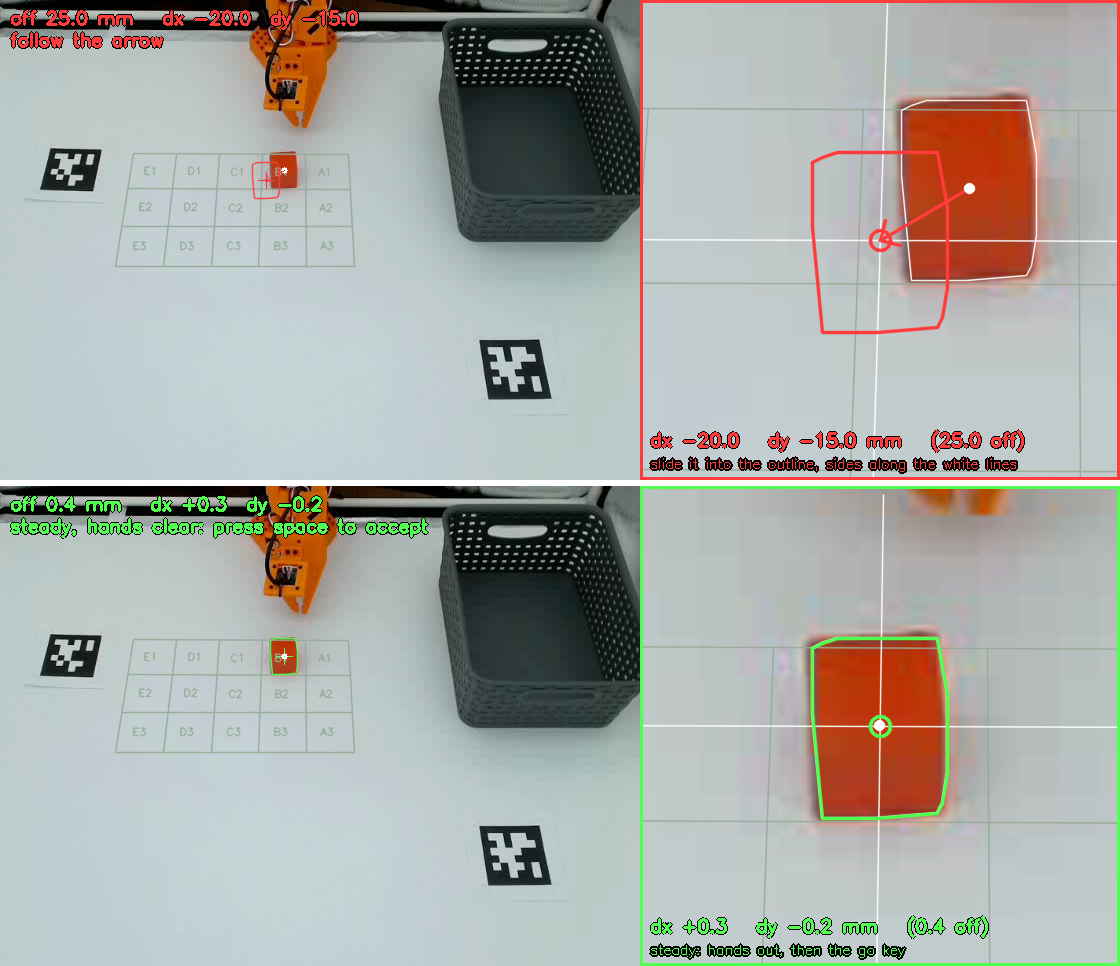
\includegraphics[width=0.82\textwidth]{figures/fig5-overlay-example.png}
\caption{The placement overlay as the operator sees it, rendered afterwards with the session's own code from the first frame of a counted trial's video. Left: the front camera's image with the grid (which is not marked on the floor) and its cell names, the two floor tags, the arm at its start pose and the basket. Right: the surroundings of the target, magnified. Top: the cube 25~mm from a target chosen for this illustration; the outline shows where the cube belongs, and the readout gives the offset in table millimetres. Bottom: the same frame against the trial's own target, within tolerance (0.4~mm from it).} % src: scripts/make_overlay_example.py and its output of 2026-10-09 (trial T1a-001: 25.0 mm from the shown target, 0.4 mm from the planned one)
\label{fig:overlay}
\end{figure*}

\emph{The table frame: tags, grid and registration.}
The grid is virtual: nothing is drawn on the floor, so that the policy sees no marks of position. The cameras see only the floor, two fiducial tags and the basket, and the grid appears in the overlay alone (Fig.~\ref{fig:overlay}). % src: protocol/protocol.md, section 3 ("The grid ... is virtual: nothing is drawn on the floor"); the reason as the operator gave it on 2026-10-09 (docs/journal.md): no record of the design days states it
Two AprilTags (Table~\ref{tab:rig}) are taped to the floor outside the grid, one in front on the right of the arm and one at the rear on the left, and tie the grid to the floor. % src: docs/runbook/00-table-layout.md, step 1 (tag 0 front right, tag 1 rear left)
Their positions in the grid's frame were measured once, in a \emph{registration}: a printed sheet carrying the grid's outline and six 36~mm tags was laid where the grid should be, the conversion from pixels to table millimetres was fitted through the six tags over 40 frames, the corners of the two floor tags were stored in that frame, and the sheet was removed. % src: config/table_geometry.json, registration (method, sheet_tags, frames); protocol/protocol.md, section 7
Two findings from the first evening shaped this design. First, a frame solved from the two floor tags alone is fragile: one pixel on one tag corner moves the far side of the grid by up to 2.5~mm, so the two tags are used to carry a frame that six tags established, and not to establish it. % src: analysis/instrument/first_sitting.md, section 3 (2.51 mm); protocol/protocol.md, section 7 ("a watchman, not a ruler")
Second, the tag detector's corners lie about 0.6 pixels inside a tag's outline at this view (about one pixel per millimetre) and move with the image's brightness, so every tag is measured by lines fitted to its outline instead. % src: config/table_geometry.json, registration.detector_inset_px (0.56); analysis/instrument/first_sitting.md (0.61 px); protocol/protocol.md, section 7
Because the camera hangs from the light box's frame, which the box's walls move (closing one zipper turned the camera by 0.1 degrees), each session solves the conversion again from the two floor tags as it finds them. % src: protocol/protocol.md, section 7 ("every session solves it afresh"); docs/runbook/00-table-layout.md, step 2 (the zipper, 0.1 degrees)

\emph{How the frame performed.}
At the registration, the six sheet tags fitted one plane to 0.41~mm on average (0.88~mm at most); a tag left out of the fit was predicted by the other five to 0.61~mm on average (1.91~mm at most); and the sheet's printed grid lines, which no fit uses, lay 0.28~mm (root mean square) from the fitted frame. % src: config/table_geometry.json, registration: sheet_fit_mean_mm 0.41, sheet_fit_max_mm 0.876, leave_one_out_mean_mm 0.613, leave_one_out_max_mm 1.914, sheet_lines.rms_mm 0.284
In use, the checks reported in Section~\ref{sec:instrument} and Table~\ref{tab:rigb} apply: steps of 10~mm were read to \instrumentMeanAbsError~mm on average, repeated readings of one position stayed within \repeatabilityScatter~mm, and accepted placements were a median of \resetErrorMedian~mm from their targets. % src: protocol/protocol.md, section 7 (the step of the scale check)
The weak point was the camera's mounting, not the tags: at the start of the six sessions with counted trials the camera's image stood 0.4 to 1.7~mm from the stored calibration, the two floor tags read 1.6 to 1.8~mm against each other relative to the registration (the rest of the image had moved with them, which indicates a rotation of the camera and not a tag's movement), and two sessions ended on the rule that allows no attempt once the image has moved more than \viewCreptLimit~mm within a session. % src: docs/decisions.md, 2026-10-08 (the six counted sessions' kept start frames read again on 2026-10-08: the camera 0.37 to 1.70 mm; the tags 1.6, 1.7, 1.8, 1.8, 1.7 and 1.8 mm, said beyond 1.5 and refused beyond 3); protocol/protocol.md, section 7 (the tags' reading follows the camera's turn); docs/journal.md, 2026-10-08 (the sessions of 13:21 and 15:38 ended by the creep rule)
A camera mount that is independent of the enclosure would remove that cost.

\emph{The instrument.}
The front camera detects the cube and converts its position to table millimetres. Each session solves this conversion from the outlines of the two floor tags, averaged over 20 frames, and measures through it; the start position of a demonstration is measured through the tags as that episode's first frame shows them. % src: protocol/protocol.md, section 7 ("The frame is the floor tags', and every session solves it afresh")
A calibration stored once serves as a reference only: a session reports a difference above 1.5~mm from it and stops above 5~mm. % src: protocol/protocol.md, section 7
The detector reports the centre of the cube's visible outline (its top and lit sides) mapped through the table plane, not the centre of its footprint.
The same holds for every demonstration and every trial, so the offset cancels in a distance, but only up to a scale factor, which geometry places a few percent above one.
Over its \nScaleRuns runs the scale check gave a factor, each run's measured length divided by its true length (50 to 150~mm), between \scaleFactorMin and \scaleFactorMax (mean \scaleFactor). % src: analysis/report/report.md, "Scale check" (runs of 60, 50, 150 and 50 mm)
The rule fixed in advance: if the runs agree within one percentage point, every distance in the analysis is divided by the mean factor; otherwise, distances are left as measured and the range of the factor is reported as the instrument's accuracy.
A placement (Fig.~\ref{fig:overlay}) is accepted when the cube is steady within \placementTolerance~mm of its target and the operator, with hands out of the camera's view, presses a key; only then can the arm move, and the position at that moment is the measured start.
For repeatability, the cube was pushed \nRepeatability times against a fixed stop and lifted away between readings; the readings stayed within \repeatabilityScatter~mm of their mean.
No overlay was involved, so this figure describes the detector alone. % src: protocol/protocol.md, section 7, item 2 ("A stop, not the overlay"); data/instrument/repeat_20261008_174537.csv

\emph{Resets by eye.}
For each of \nByEye targets, the cube was returned to its position using a reference image shown beside the live view, with no overlay and no readout.
Number of people who placed the cube by eye: \nOperatorsByEye; the largest error was \byEyeErrorMax~mm.
This corresponds to an evaluation that resets the object ``to the same place'' from an image or from memory.
It does not correspond to an evaluation that overlays a reference image on the live view; we did not measure that case and expect its error to lie between that of resets by eye and that of the resets of this study.

\emph{Recording.}
One operator recorded both sets on one day with the same task text, time limit, cube orientation (square to the grid), start pose, approach side and grasp, in rounds of one episode per trained cell in shuffled order; an episode ended when the operator pressed a key, so episodes differ in length (Table~\ref{tab:rigb}). % as recorded: data/recording/*_placements.jsonl (ten rounds of 11 episodes, 11 distinct trained cells each, on 2026-10-07); data/audit/*_rate.json (17 to 26 s)
An episode was recorded again when the operator made a handling error, the cube was outside tolerance or a check failed.
The protocol plans a practice block that is recorded and discarded; the procedure of the recording day asks for practice without recording, and the logs hold no practice episode. % src: protocol/protocol.md, section 4 ("A practice block of about 10 episodes is recorded first and discarded"); docs/runbook/02-arm-and-recording.md, step 4 (practice, nothing recorded); data/recording/*_placements.jsonl
The clustered layout repeats each location to within about a millimetre: the \nDemosPerCell start positions at a location are within \clusteredScatterMax~mm of their mean.
In our earlier dataset, where the cube was placed using a grid drawn over the camera image and the start positions were not measured, the two farthest of a cell's five demonstrations were 4.8 to 13.7~mm apart, so a location repeated without a measuring aid is itself somewhat spread. % src: protocol/protocol.md, section 4 ("This clustered set is tighter than August's"); analysis/pilot_august/README.md (4.8 mm in cell A3 to 13.7 mm in cell D1, through one conversion)
The two layouts compared here are therefore the two extremes of a range; a recording made without a placement aid lies between them.
Before training, each dataset was checked for its episode and frame counts, the decoding of both camera streams, frame pacing and torn frames (Appendix~\ref{app:faults} reports the results of the last two), and by the start-state audit: every episode in its planned cell and within 3~mm of its target. % src: protocol/protocol.md, section 4 (dataset checks before training)

% ======================================================================================================================
\section{The protocol: predictions, analysis and stop rules}
\label{app:protocol}
The protocol (version \protocolVersion) was frozen before the first counted trial. % src: config/protocol.toml (version 1.0, status frozen); git tag protocol-v1, 2026-10-08 12:50:13; the first counted trial began at 13:22:47
A \emph{counted} trial is one run under the frozen protocol, and only counted trials are analysed.
Before the freeze, \emph{pilot} trials tested the procedure: a replay pilot, and nine exact repeats with the clustered policy (the second stop rule below). % src: protocol/protocol.md, sections 8 and 12
Pilot trials were written to separate logs, and the trial runner does not start a counted trial until the protocol is frozen.
The predictions below were written three days before the first counted trial and two before the first pilot trial, and were not changed after the day they were written. % src: git history of protocol/protocol.md: section 9 at tag protocol-v1 is word for word that of commit ce89dba (2026-10-05 20:53); the workspace test's placements, which prediction 3 is about, were last changed that evening too (draft 0.3, commit 8c22c0a, 22:58); the first pilot trial is of 2026-10-07 17:24 (data/trials/pilot_shakedown.jsonl)

\subsection{Predictions stated before the data}
Every radius in this list is a block fit (defined below).
\begin{enumerate}
\item \emph{The curve.} The clustered policy succeeds at least 5 times in \anchorsZeroClustered at $d=0$ and at most once in \anchorsFarClustered at \farLevel~mm, and its radius lies between 5 and 40~mm. % src: protocol/protocol.md, section 9, prediction 1
\emph{Observed:} \successZeroClustered of \nZeroClustered, \successFarClustered of \nFarClustered, and \radiusClusteredThreshold~mm (\radiusClusteredThresholdLow to \radiusClusteredThresholdHigh). Only the median met the prediction: the interval extends to \radiusClusteredThresholdHigh~mm, and the median of the second fit of the plateau check, \radiusClusteredThresholdWide~mm, lies outside the predicted range (Table~\ref{tab:plateau}).
\item \emph{Hardware.} The policy's radius is larger than the replay's, by the rule for ``larger'' below.
\emph{Observed:} a difference of \radiusDiffClusteredReplay~mm (\radiusDiffClusteredReplayLow to \radiusDiffClusteredReplayHigh), and a posterior probability $\probClusteredExceedsReplay$ that the policy's radius is the larger. The prediction was met under the pre-specified rule; the policy's radius itself is not established.
\item \emph{Layout.} At the placements of the workspace test, the spread policy succeeds more often than the clustered one. % src: protocol/protocol.md, section 9, prediction 3 (its wording; where the placements are drawn is in "The blocks as planned")
\emph{Observed:} \workspaceSuccessSpread against \workspaceSuccessClustered of \nPairs ($p=\mcnemarP$). The prediction was not met: the counts are in the predicted direction, but the test does not establish a difference.
\item \emph{Lookup.} Each policy's success in the workspace test matches the lookup prediction: its observed count lies inside the prediction's \intervalLevel~\% interval.
\emph{Observed:} \workspaceSuccessClustered against a predicted \lookupPredictedClustered (\lookupClusteredLow to \lookupClusteredHigh) for the clustered policy, and \workspaceSuccessSpread against \lookupPredictedSpread (\lookupSpreadLow to \lookupSpreadHigh) for the spread policy. The prediction was met, with wide intervals and conditional on the curve from which it is computed.
\item \emph{Layout and radius.} No prediction; reported as an estimate.
\emph{Observed:} not available. The spread policy's threshold block was not run (Appendix~\ref{app:counts}), so it has no block fit and the two radii are not compared; its workspace-test trials alone bound its radius from below, at \radiusSpreadLow~mm.
\end{enumerate}

\subsection{The blocks as planned}
Table~\ref{tab:design} gives each block.
Staircases move in steps of \stepInitial~mm until their first reversal and \stepFinal~mm after it, between 0~mm and the block's largest distance; the replay's may request up to \maxLevelReplay~mm. % src: config/protocol.toml, staircase.min_level_mm
A requested distance is met when the target's distance to its nearest demonstration is within \levelMatch~mm of it, and test placements keep the cube's centre at least \testMargin~mm inside the grid's edge.
For a replay the target is drawn uniformly in direction on the circle of that radius around the start of the demonstration played back.
The held-out cells are \heldOutCells.
Inside a trained cell no point is farther than about \clusteredMaxDistInCell~mm from a clustered demonstration, or than about 17~mm from a spread one; larger distances are tested in held-out cells. % src: protocol/protocol.md, section 4 (largest gap of the planned spread layout: 17.2 mm; of the clustered one: 35.4 mm)
The far anchor trials are set at \farLevel~mm and not at \maxLevelClustered~mm, where nearly every admissible point lies in a corner cell; at \farLevel~mm the two interior held-out cells also contain admissible points.
The workspace test draws \nPairsTrainedPlanned of its \nPairsPlanned placements uniformly over the trained cells and \nPairsHeldOutPlanned over the held-out cells, and tests them in one shuffled order.
With placements in trained cells only, the paired test could detect no difference once the radius is large enough for the clusters to cover their own cells; with placements in held-out cells only, it could detect none while the radius is small. A calculation under the lookup model, made before any trial, was used to choose the design. % src: protocol/protocol.md, section 8, and analysis/simulation/workspace_designs.md (the designs compared, and how often each would reach p < 0.05)
Both policies were to be evaluated at step \trainSteps; had a run not reached it in time, both would have been evaluated at their largest common saved step, and not below \trainStepsFallback.

\emph{The replay.}
The replay block plays back \nReplayDemosPlanned demonstrations of the clustered set, one from each trained cell, so that the replay is tested over the same regions of the table as the policy; the planner's seed draws which of a cell's \nDemosPerCell it is, before any trial.
The block's \plannedReplay trials replay each demonstration twice, in two different parts of the block: the \anchorsZeroReplay trials at $d=0$ are \anchorsZeroReplay different demonstrations, and each staircase replays \stairTrialsReplay different ones. % src: protocol/protocol.md, section 6 ("twice" holds because the block has two trials for each demonstration; a test of config/protocol.toml holds it to that)
Which demonstration a trial replays does not depend on any outcome.
In the replay pilot, each of the \nReplayDemosPlanned demonstrations was replayed once from its own start position: ten succeeded, and the eleventh attempt was terminated by an accidental key press and is logged as a failure. % src: data/trials/pilot_replay.jsonl (the 11 trials at level 0: 10 successes; T1b-022, note "accidental keyboard type", 5.7 s); protocol/protocol.md, section 6 asks for this count
The safety gate that transfers control of the motors allows a replay to begin only when every joint is within \handoffToleranceReplay degrees of that demonstration's first recorded action, so a replay starts from approximately the pose from which the demonstration started.
A policy trial has a looser tolerance of \handoffTolerance degrees: the policy observes the arm and may start from any nearby pose.

\emph{Order and blinding.}
The trials of the clustered policy's block and of the replay block, \plannedClustered and \plannedReplay, are shuffled into one seeded order, so that the policy and the replay are tested at the same time of day, at the same servo temperature and in the same state of the cameras.
The workspace test follows, with the two trials of a pair in immediate succession on the same target and each policy first in half of the pairs; the spread policy's block was planned last and was not run.
As run, the interleaved order took four consecutive sessions in about 91 minutes: one session was ended by the rule on camera movement (Table~\ref{tab:rigb}) and two after the arm had displaced the basket (see below). The workspace test followed 47 minutes later, in two sessions, the first of which was ended by the same rule; no pair was split between sessions. % src: data/trials/main.jsonl (ts_start, media folders, notes); docs/journal.md, 2026-10-08
A trial is identified to the operator by a running number and a code drawn from one shuffled list.
Neither indicates which policy runs, which block the trial belongs to, or whether it is a replay.

\emph{The second scoring.}
Every attempt was recorded on video by both cameras.
After the last trial, one scored trial in five of each condition of each block (\nSecondScored of \nTrialsTotal) was drawn by a seed and the hash of the trial log itself, so that it could not be known in advance which trials would be scored again; the two trials of a workspace pair were never both drawn. % src: protocol/protocol.md, section 8 ("A second scoring from video")
These trials were scored again from the videos alone, under neutral names and in shuffled order, with no condition, distance or first score shown.
No second person was available, so the operator who had scored at the rig gave both scores.
The two scores agree in \nSecondScoredAgree of \nSecondScored trials; in \nSecondScoredCannotTell trials the video did not show the outcome.
The score given at the rig remains the trial's outcome regardless of the second score.

\emph{Void trials and failures.}
A trial is void when it could not test its condition: the placement was later found outside tolerance, a camera or motor fault ended the attempt, a person interfered, the safety gate refused the start three times, or a key press ended the attempt within one second of its start.
A void trial remains in the log with its reason, and its position in the plan is repeated with the same target, under a new number and a new code. % src: protocol/protocol.md, section 8 (the five reasons)
A stop caused by the condition's own motion after the handover (the per-step clamp, the stall rule) is a failure.

\emph{The basket and the wrist camera.}
The basket is fixed to the floor with double-sided tape. At a release, the wrist camera's mount can strike the basket's rim and displace it, and the same contact can shift that camera in its mount.
A trial in which this happens keeps its score; the basket is then repositioned with a live overlay of a reference image, and the wrist camera's position is read from the position of the gripper's fixed jaw in its image.
The first frames of each trial's own videos were read afterwards. The arm displaced the basket by more than 5~mm in \nTrialsBasketMoved trials (by 35 and 45~mm). In \nTrialsBasketNamed trials the basket began more than 2~mm from its reference position, in all of them between 2.1 and \basketStartMax~mm: one pixel is about 1.1~mm there, so these readings are two pixels from the reference. The number of trials that began with the jaw more than 2 pixels from its position in training was \nTrialsWristNamed (\wristStartMax pixels at most; the camera's view was offset by about 2 pixels before the first block and was not corrected). The analysis report lists the trials by identifier. % src: protocol/protocol.md, section 8 (the two limits); data/audit/scene_main.json (basket_moved_mm of the two trials; the start readings); src/tolerance_radius/rig/basket_place.py, MM_PER_PX (1.08); docs/decisions.md, 2026-10-08 (the wrist camera is left where it stands)

\begin{table}[t]
\caption{The blocks as planned. Distances in millimetres.}
\label{tab:design}
\centering
\footnotesize
\setlength{\tabcolsep}{4pt}
\begin{tabular}{@{}lcccc@{}}
\toprule
 & Trials & Trials at & Two staircases: & Largest \\
Block & at $d=0$ & \farLevel~mm & starts; trials each & distance \\
\midrule
Replay & \anchorsZeroReplay{} & -- & \stairStartNearReplay{} and \stairStartFarReplay{}; \stairTrialsReplay{} & \maxLevelReplay{} \\
Clustered policy & \anchorsZeroClustered{} & \anchorsFarClustered{} & \stairStartNearClustered{} and \stairStartFarClustered{}; \stairTrialsClustered{} & \maxLevelClustered{} \\
Spread policy & \anchorsZeroSpread{} & -- & \stairStartNearSpread{} and \stairStartFarSpread{}; \stairTrialsSpread{} & \maxLevelSpread{} \\
Workspace test & \multicolumn{4}{l}{\nPairsPlanned placements, each with both policies:} \\
 & \multicolumn{4}{l}{\nPairsTrainedPlanned in trained cells, \nPairsHeldOutPlanned in held-out cells} \\
\bottomrule
\end{tabular}
\end{table}

\subsection{Analysis fixed in advance}
\begin{itemize}
\item \emph{Model and estimate.} Eq.~\eqref{eq:model}, with a posterior on a grid: a flat prior on $r_{50}$ from 0 to \gridRadiusMax~mm in steps of 0.5~mm, a flat prior on $\log w$ over 30 values from \gridWidthMin to \gridWidthMax~mm, and $\lambda\in\{\lapseValues\}$ and $\gamma\in\{\floorValues\}$, the values of each equally weighted. % src: config/protocol.toml, analysis.r50_grid_mm (min, step) and analysis.width_grid_mm.count
We report the posterior median of $r_{50}$ and its equal-tailed \intervalLevel~\% interval.
The staircases only choose where to test.
\item \emph{Rationale for the floor.} A trial far from every demonstration can still succeed by chance.
In the earlier evaluation one did, through a grasp at the cube's edge at 40~mm, and with the floor fixed at zero that single trial changed the fitted radius from 19.5 to 26~mm. % src: analysis/pilot_august/README.md, "Where the 50 % point can be" (the model of protocol draft 0.1, without a floor; trial 28)
The floor values limit the influence of such a success on the radius.
They do not measure how often chance successes occur; the far anchor trials give that as a count.
\item \emph{An interval that is open on a side.} The interval is \emph{open} on a side when the posterior at that end of the grid is at least half of what it is at the interval's own bound on that side.
We then report ``at most'' the upper bound (open below) or ``at least'' the lower bound (open above), and not a radius.
This occurs when success is already decreasing at $d=0$, or is still on its plateau at the largest distance tested.
\item \emph{The plateau is checked.} The lapse values above stop at 0.10, which suits a condition that nearly always succeeds at a demonstration's own start. % src: config/protocol.toml, analysis.lapse_values (the largest)
With a lower plateau the model would account for failures near a demonstration by a smaller radius: in simulation, a true plateau of 0.65 reduced the estimated radius by 8~mm. % src: protocol/protocol.md, section 10 (analysis/simulation/lapse_values.md); simulated, not measured
Every fit is therefore made a second time with $\lambda\in\{\lapseValuesWide\}$, and both fits are reported with the counts at $d=0$ (Table~\ref{tab:plateau}).
The first fit gives the radius we report. If the two medians differ by more than \plateauShiftLimit~mm, we state that the condition's plateau is uncertain and its radius not established, and every result that depends on that radius (a comparison, the lookup prediction, the reset sensitivity, prediction 1) is still computed by its rule and reported with that caveat. % src: protocol/protocol.md, section 10 (what rests on a radius; "prediction 1" is the first item of the list above)
Here the clustered policy's pooled fit changed by \plateauShiftClustered~mm, so the caveat applies to this policy; its block fit changed by \plateauShiftClusteredThreshold~mm.
Over all 60 of its scored trials, the policy succeeded in all 11 trials within 10~mm of a demonstration, in 6 of 10 between 10 and 20~mm, and in 9 of 12 between 30 and 40~mm (all of the latter in held-out cells): the decline is gradual and location matters besides distance (Section~\ref{sec:results}), which a single curve of distance does not represent. % src: analysis/report/report.md, "Clustered policy", the table of 10 mm bins over its 60 scored trials
\item \emph{Two fits.} The \emph{block fit} uses a condition's own threshold block only.
Every comparison and every prediction uses block fits: the comparison of the policy with the replay, two blocks of one session, and the lookup prediction, which must not have seen the workspace-test trials it predicts.
The \emph{pooled fit} adds a policy's workspace-test trials at their measured distances, and is reported alongside the block fit as a check that the two agree.
The spread policy's threshold block was not run, so it has a pooled fit only, from its workspace-test trials: placements fixed in advance and not chosen by a staircase, half of them in held-out cells.
\item \emph{The radius as the reported quantity.} We report $r_{50}$ and not $w$: thresholds need far fewer trials than slopes \cite{kontsevich1999bayesian}, and slopes fitted to adaptive data are biased \cite{kaernbach2001slope}.
\item \emph{Without a model.} Success counts in 10~mm bins of $d$, closed below and open above, with Wilson intervals \cite{wilson1927probable}; the largest $d$ with a success and the smallest with a failure. % src: protocol/protocol.md, section 10
\item \emph{Comparison of radii.} The posterior probability that one condition's $r_{50}$ exceeds another's, from the two block fits taken as independent, and the difference with its interval.
``Larger'' means a probability of at least 0.95 and ``smaller'' one of at most 0.05; anything between is reported as not distinguished by these trials. % src: protocol/protocol.md, section 9, prediction 2
\item \emph{Workspace test.} The table of paired outcomes, the exact McNemar test, and each policy's success with a Wilson interval.
All placements make one test; the counts for trained and for held-out cells apart, a pair counting by the cell its cube was measured in, are descriptive.
We call the two policies different at these placements when the test's two-sided $p$ is below 0.05, the level at which we state below what the test can show. % src: protocol/protocol.md, section 9, prediction 3 (the rule: the exact paired test, p below 0.05) and section 8
\item \emph{Lookup prediction.} For each placement and policy, the predicted probability of success is the clustered policy's block fit at that placement's measured distance to the policy's own nearest demonstration, averaged over the posterior.
We report the expected number of successes, the \intervalLevel~\% interval of the predicted count, which carries both the uncertainty of the fit and the chance in \nPairsPlanned trials, the observed count, and whether it lies inside.
The fit comes from a block run earlier in the day, so a change in the rig between the two would also appear as a mismatch.
\item \emph{Reset sensitivity.} The success the clustered policy's block fit gives at trained positions if resets carry the by-eye errors, beside the same calculation with this study's own placement errors. A calculation, not a measurement.
The curve is evaluated at a distance equal to each of the \nByEye by-eye errors, and to each of the \nTrialsTotal placement errors of the scored trials, and the results are averaged. The result: \resetSensitivityByEye~\% with the by-eye errors against \resetSensitivityPlaced~\% with this study's placement errors, conditional on a fitted curve whose radius is not established; it does not apply to resets made with an overlay.
\item \emph{Descriptive only.} Success by placement inside or outside the convex hull of the demonstrations; failure labels by distance; durations; the achieved control rate.
\item \emph{Exclusions.} No trial is excluded except void trials and pilot trials, and no outcome is changed after the fact.
\end{itemize}

\begin{table}[t]
\caption{The plateau check: each fit made with the lapse values of the analysis (up to 0.10) and again with the longer list (up to 0.50). Posterior median and \intervalLevel~\% interval of $r_{50}$ in millimetres; an interval that the data do not bound above is given as its lower bound, and the median of such a fit is shown only to give the shift, which is the second median minus the first. The second column gives the successes at $d=0$ among the fit's trials.} % src: config/protocol.toml, analysis.lapse_values and analysis.lapse_values_sensitivity (their largest values)
\label{tab:plateau}
\centering
\footnotesize
\setlength{\tabcolsep}{1.8pt}
\begin{tabular}{@{}lcccccc@{}}
\toprule
 & At & \multicolumn{2}{c}{$\lambda\le 0.10$} & \multicolumn{2}{c}{$\lambda\le 0.50$} & \\ % src: the same two lists
Fit & $d=0$ & median & interval & median & interval & Shift \\
\midrule
Replay, block & \successZeroReplay{}/\nZeroReplay{} & \radiusReplay{} & \radiusReplayLow{}--\radiusReplayHigh{} & \radiusReplayWide{} & \radiusReplayWideLow{}--\radiusReplayWideHigh{} & \plateauShiftReplay{} \\
Clustered, block & \successZeroClustered{}/\nZeroClustered{} & \radiusClusteredThreshold{} & \radiusClusteredThresholdLow{}--\radiusClusteredThresholdHigh{} & \radiusClusteredThresholdWide{} & $\geq$\,\radiusClusteredThresholdWideLow{} & \plateauShiftClusteredThreshold{} \\
Clustered, pooled & \successZeroClustered{}/\nZeroClustered{} & \radiusClustered{} & \radiusClusteredLow{}--\radiusClusteredHigh{} & \radiusClusteredWide{} & \radiusClusteredWideLow{}--\radiusClusteredWideHigh{} & \plateauShiftClustered{} \\
Spread, pooled & none & \radiusSpread{} & $\geq$\,\radiusSpreadLow{} & \radiusSpreadWide{} & $\geq$\,\radiusSpreadWideLow{} & \plateauShiftSpread{} \\
\bottomrule
\end{tabular}
\end{table}

\subsection{What the trial budget can show}
Before the freeze we simulated each threshold block against success curves assumed true and fitted it as the analysis fits the real trials (\simReplications simulated blocks for each curve).
Every figure in this subsection is simulated or computed from stated assumptions; none is a measurement.

\emph{One radius.}
For the clustered policy's block and an assumed curve with $r_{50}=\simTruthRadius$~mm and $w=\simTruthWidth$~mm, the estimated radius differed from the true radius by \simBias~mm on average, with a root-mean-square error of \simRmse~mm; its interval was \simIntervalWidth~mm wide on average and held the true radius in \simCoverage~\% of blocks.
The same number of trials at fixed, equally spaced distances gave an error of \simRmseConstant~mm and an interval \simIntervalWidthConstant~mm wide, which is why the staircases were kept.
The precision depends on how steep the true curve is, which is not known before the trials: Table~\ref{tab:simblocks} gives each threshold block's simulated error and interval width for a steep curve ($w=\simWidthCliff$~mm), an intermediate one ($w=\simWidthMiddling$~mm) and a shallow one ($w=\simWidthSlope$~mm).
Where success is already decreasing at $d=0$, the interval was open below in \simOpenBelow~\% of simulated blocks: the estimate is then reported as ``at most'' and not as a radius.
\begin{table}[h]
\caption{Simulated before any trial: root-mean-square error of the estimated radius / mean width of its \intervalLevel~\% interval, in millimetres, for each threshold block as planned and three widths of the assumed curve. These values are simulated, not measured.}
\label{tab:simblocks}
\centering
\footnotesize
\begin{tabular}{@{}lccc@{}}
\toprule
Block & Steep & Intermediate & Shallow \\
\midrule
Clustered policy & \simRmseClusteredCliff{} / \simIntervalWidthClusteredCliff{} & \simRmseClusteredMiddling{} / \simIntervalWidthClusteredMiddling{} & \simRmseClusteredSlope{} / \simIntervalWidthClusteredSlope{} \\
Replay & \simRmseReplayCliff{} / \simIntervalWidthReplayCliff{} & \simRmseReplayMiddling{} / \simIntervalWidthReplayMiddling{} & \simRmseReplaySlope{} / \simIntervalWidthReplaySlope{} \\
Spread policy & \simRmseSpreadCliff{} / \simIntervalWidthSpreadCliff{} & \simRmseSpreadMiddling{} / \simIntervalWidthSpreadMiddling{} & \simRmseSpreadSlope{} / \simIntervalWidthSpreadSlope{} \\
\bottomrule
\end{tabular}
\end{table}

\emph{Two radii.}
How large a difference between the policy's radius and the replay's radius the rule for ``larger'' can detect depends on how steep the two curves are, and the rule can also err when the two radii are equal.
Table~\ref{tab:simrule} gives, for a replay radius of \simRuleReplayRadius~mm and \simRulePairs simulated pairs of blocks per case, how often the rule returned ``larger''.
At equal radii it returned ``larger'' in \simRuleLargerWidthThreeDiffEqual~\% of pairs and ``smaller'' in \simRuleSmallerWidthThreeDiffEqual~\% (both curves of width \simWidthMiddling~mm).
\begin{table}[h]
\caption{Simulated before any trial: share of pairs of blocks (clustered policy, replay) in which the rule returned that the policy's radius is the larger, in percent, by the true difference of the two radii and the width of both curves. These values are simulated, not measured.}
\label{tab:simrule}
\centering
\footnotesize
\setlength{\tabcolsep}{4pt}
\begin{tabular}{@{}lcccccc@{}}
\toprule
Width & equal & +3~mm & +5~mm & +8~mm & +10~mm & +15~mm \\ % src: analysis/simulation/comparison_rule.md, the cases simulated
\midrule
1~mm & \simRuleLargerWidthOneDiffEqual & \simRuleLargerWidthOneDiffThree & \simRuleLargerWidthOneDiffFive & \simRuleLargerWidthOneDiffEight & \simRuleLargerWidthOneDiffTen & \simRuleLargerWidthOneDiffFifteen \\ % src: analysis/simulation/comparison_rule.md, the cases simulated
3~mm & \simRuleLargerWidthThreeDiffEqual & \simRuleLargerWidthThreeDiffThree & \simRuleLargerWidthThreeDiffFive & \simRuleLargerWidthThreeDiffEight & \simRuleLargerWidthThreeDiffTen & \simRuleLargerWidthThreeDiffFifteen \\ % src: analysis/simulation/comparison_rule.md, the cases simulated
6~mm & \simRuleLargerWidthSixDiffEqual & \simRuleLargerWidthSixDiffThree & \simRuleLargerWidthSixDiffFive & \simRuleLargerWidthSixDiffEight & \simRuleLargerWidthSixDiffTen & \simRuleLargerWidthSixDiffFifteen \\ % src: analysis/simulation/comparison_rule.md, the cases simulated
\bottomrule
\end{tabular}
\end{table} % src: analysis/simulation/comparison_rule.md; the column heads are that report's cases

\emph{Two policies at the same placements.}
With \nPairsPlanned pairs and true success rates of \simPairedRateLow and \simPairedRateHigh~\%, the exact McNemar test reaches $p<0.05$ in \simPairedPower~\% of cases, by an exact sum that takes the two outcomes at a placement as independent. % src: the level the procedure simulation uses for its power table
It cannot reach that level with fewer than six discordant pairs, and with six only if all six favour the same policy. % src: arithmetic, two-sided exact test: 2 x 0.5^6 = 0.031, and 2 x 0.5^5 = 0.0625
The test therefore detects only large differences; where the two policies are closer, we can report only the counts and their intervals.

\subsection{Stop rules}
Table~\ref{tab:stops} gives the criteria fixed in advance.
What happened at each is as follows.
\emph{Before recording:} the scale check passed (Section~\ref{sec:instrument}) and the camera's reference was stored. The rig check passed its five steps on the arm and the cameras and failed its last step, a comparison of the front camera's image with a stored one, on a stream that had opened without the manually set exposure; the image matched the stored one again a minute later. No complete pass of that check was recorded afterwards, and the rule for a missed line (omit the spread set) was not applied: both sets were recorded the next day. From then on every session, and the recorder at every episode, compared the image's white and black levels with those of the stored calibration before proceeding. This happened two days before the protocol was frozen, so it is reported here and is not among the deviations from the frozen protocol. % src: docs/journal.md, 2026-10-06 (the rig check's sixth step, and the frame a minute later); analysis/report/report.md, "Scale check"
\emph{After recording:} both datasets passed their audits, and the pilot gave 8 successes in 9 exact repeats (trials at a demonstration's own start), the minimum required. % src: data/audit/clustered.json and spread.json; data/trials/pilot_policy.jsonl (9 scored trials at 0 mm, 8 successes)
\emph{During the trials:} the two interleaved blocks were complete at 14:54, before the set time of 15:00. % src: data/trials/main.jsonl (the last trial of blocks T1a and T1b); protocol/protocol.md, section 12
\emph{End of the trials:} those two blocks and the workspace test were complete. The spread policy's block was then omitted by a decision of the operator and not under the third criterion; it is the first deviation listed in Appendix~\ref{app:counts}. % src: docs/decisions.md and docs/journal.md, 2026-10-08

\begin{table}[t]
\caption{Stop rules fixed before the experiment.}
\label{tab:stops}
\centering
\footnotesize
\begin{tabular}{@{}p{0.16\columnwidth}p{0.39\columnwidth}p{0.32\columnwidth}@{}}
\toprule
When & Pass criterion & If missed \\
\midrule
Before recording & Rig check passes; camera baseline stored; scale check within 1.5~mm mean absolute error, no step deviating by more than 3~mm & Repair before recording; if that is not possible in time, omit the spread set \\ % src: protocol/protocol.md, sections 7 and 12
After recording & Both datasets recorded and audited; in a pilot, a clustered checkpoint succeeds in at least 8 of 9 exact repeats & Stop: no submission \\ % src: protocol/protocol.md, section 12
During the trials & The clustered policy's block and the replay block complete by a set hour & Skip the spread policy's block; run the workspace test only if all its pairs fit \\
End of the trials & The clustered policy's block and the replay block complete & Report the completed blocks, and state what was planned and not run \\
\bottomrule
\end{tabular}
\end{table}

% ======================================================================================================================
\section{Deviations, trial counts and void trials}
\label{app:counts}
The decision log records \nDeviations deviations from the frozen protocol. % src: docs/decisions.md, the three rows of 2026-10-08 marked as deviations; protocol/protocol.md, section 13
First, the spread policy's threshold block (\plannedSpread trials) was planned and not run. The protocol's rule for omitting it applies when the two interleaved blocks are not complete by a set time, and they were; the operator omitted it on the day of the trials, to allocate the remaining time to the by-eye resets, the repeatability check and the second scoring. At that point the operator had scored every trial without knowing its condition, and no count by condition had been computed. As a consequence the spread policy has no threshold block, and the two policies' radii are not compared. % src: protocol/protocol.md, sections 8 and 12; docs/decisions.md and docs/journal.md, 2026-10-08
Second, the repeatability check, which the protocol places before any trial, was run after the last trial on the same day.
Third, the check of the camera against the floor tags that the protocol places at the end of each block was not run as a separate step: the start of the next session, about 47 and 39 minutes after the last trial of the two blocks, made the same check, and both passed (0.8 and 0.7~mm from the stored calibration, where a session stops above 5~mm). % src: docs/decisions.md, 2026-10-08 (the two sessions' kept start frames, read again: 0.82 and 0.71 mm)
The second and third do not change what any trial measured.
Table~\ref{tab:counts} gives the trials planned, scored and void in each block.
Void trials: \voidReasons.
Of the descriptive results planned (Appendix~\ref{app:protocol}): every failure carries the label ``grasp'': 23 for the clustered policy (at 10.1 to 50.6~mm), 9 for the replay (14.7 to 25.4~mm) and 4 for the spread policy (16.1 to 38.3~mm). A trial's record lasted a median of 24~s, 24~s and 20~s, which is longer than the attempt itself. Inside the convex hull of its demonstrations the clustered policy succeeded in 28 of 36 trials and outside it in 9 of 24; the spread policy in 21 of 22 and 1 of 4. % src: analysis/report/report.md, "Descriptive only" (hull, failure labels with their ranges of d, median durations, in the order clustered policy, replay, spread policy)
Number of days on which trials ran: \nTrialDays. Number of people who placed the cube and scored: \nOperators.
Fig.~\ref{fig:workspace} shows the workspace test. In it both policies succeeded at \pairsBoth placements and neither at \pairsNeither; the placements were at most \workspaceDistClusteredMax~mm from a clustered demonstration and \workspaceDistSpreadMax~mm from a spread one.
The replay block played back \nReplayEpisodes demonstrations of the clustered set (planned: \nReplayDemosPlanned).

\begin{figure}[t]
\centering
\figureorbox{figures/fig4-workspace.pdf}{4.0cm}{The test placements on the grid, once per policy, with each policy's demonstrations, discs of the clustered policy's block-fit radius around them, and the outcome at each placement; predicted and observed counts below.}
\caption{The workspace test: each policy's demonstrations and the outcome at each of the \nPairs shared placements. In both panels the discs have the clustered policy's fitted radius $r_{50}$, which is not established; they are not a measured region of success. Below: successes and failures observed, and the successes the lookup prediction expects with its interval, for all placements and by kind of cell.}
\label{fig:workspace}
\end{figure}

\begin{table}[t]
\caption{Trials planned, scored and void, by block.}
\label{tab:counts}
\centering
\footnotesize
\begin{tabular}{@{}lccc@{}}
\toprule
Block & Planned & Scored & Void \\
\midrule
Replay & \plannedReplay{} & \nTrialsReplay{} & \nVoidReplay{} \\
Clustered policy, threshold & \plannedClustered{} & \nTrialsClusteredThreshold{} & \nVoidClusteredThreshold{} \\
Workspace test, both policies & \plannedWorkspace{} & \nTrialsWorkspace{} & \nVoidWorkspace{} \\
Spread policy, threshold & \plannedSpread{} & \nTrialsSpreadThreshold{} & \nVoidSpreadThreshold{} \\
\midrule
All & \plannedTotal{} & \nTrialsTotal{} & \nVoidTotal{} \\
\bottomrule
\end{tabular}
\end{table}

% ======================================================================================================================
\section{The earlier evaluation, re-analysed}
\label{app:earlier}
% Every number in this section is measured already. Each was recomputed on 2026-10-05 from
% analysis/pilot_august/trials_with_distance.csv, except where the line names analysis/pilot_august/README.md.
The earlier evaluation of Fig.~\ref{fig:earlier} tested one ACT policy on the same task, on this arm, with the front camera on a tripod instead of in the light box. % src: the earlier project's run journal (recording 2026-08-18 and all 31 trials on 2026-08-19 with the camera on a ground tripod; the light box from 2026-08-22). The same arm: one follower id and one calibration file, written 2026-07-03 and unchanged through this study (numbers_by_hand.tex, \rigCalibration)
Its 31 trials did not log the cube's start position. % src: trials_with_distance.csv, 31 rows
We measured it afterwards with the detector that had measured that policy's demonstrations: from the first frame of the trial's video in 30 trials, and from a still image saved at the start of the session for the one trial that was not recorded on video. % src: same file, position_source: 30 "video frame", 1 "session-start still"
The policy had been trained on 49 of the 55 demonstrations of its dataset, and distances are to the nearest of those 49. % src: analysis/pilot_august/README.md, "What was done", item 5 (read there from the earlier project's records)

The 19 trials in cells with demonstrations started 0.6 to 5.6~mm from the nearest trained demonstration, 17 of them within 3.1~mm, and all succeeded (Wilson 95~\% interval 83 to 100~\%). % src: same file, kind = id: d from 0.63 to 5.63; 17 rows at 3.03 or below; Wilson interval of 19/19 recomputed: 0.832 to 1
The 12 trials in held-out cells started 31 to 47~mm away and one succeeded, at 40~mm (1.5 to 35~\%). % src: same file, kind = ood: d from 31.01 to 47.14; the success is trial 28 at 40.01; Wilson interval of 1/12 recomputed: 0.015 to 0.354
With a second conversion from pixels to millimetres, one map for every image, the two groups are at 0.1 to 4.9~mm and at 32 to 47~mm: the untested range does not depend on the conversion. % src: same file, column d_nearest_trained49_mm_onemap: 0.11 to 4.89, and 32.46 to 46.89
In nine of the trials the cube had been placed on a demonstration's recorded start with an overlay that drew that demonstration's cube over the live view and showed the offset in pixels; those placements were 0.8 to 3.0~mm from it. % src: same file, ghost_error_mm in the 9 rows with a ghost_episode: 0.80 to 3.03

Three factors limit what that evaluation can show, in addition to the untested range.
Every near trial was in a cell with demonstrations and every far trial in a held-out cell, so it cannot separate distance from cell. % src: same file: all 19 rows with d below 10 have kind = id, all 12 above have kind = ood
The 31 trials are 12 scenes (a cell, or one demonstration's start re-created), each run two or three times, so they are not 31 independent tests and the intervals above are too narrow. % src: same file, scene_id: 12 distinct values, 2 or 3 rows each
Finally, the distances include a scale error that was not measured: the detector reads the centre of the cube's visible outline, not of its footprint, which, by geometry, makes measured distances a few percent too long. % src: analysis/pilot_august/README.md, "What these data cannot show" (an estimate from geometry, not a measurement)
The present study begins by measuring that scale.
% Not used, because it was not recomputed from the CSV (analysis/pilot_august/README.md, "How noisy the conversion is"):
% that evaluation's procedure gave its overlay tolerance of 4 pixels as "about 2 mm", and the re-analysis measured
% 4.2 to 5.3 mm. If the author verifies it, it is a direct example for the checklist's reset-accuracy entry.

% ======================================================================================================================
\section{Faults in the data pipeline of the earlier work}
\label{app:faults}
% THE COUNTS IN THIS SECTION ARE NOT IN THIS REPOSITORY. They are the \prior... macros of numbers_by_hand.tex, each copied
% from the earlier project's own records or measured again on its files; every line there says which (2026-10-08).
The earlier project's own records show three faults, each of which passes a check that the project had and each of which the project itself found within a day (Table~\ref{tab:faults}). % src: the earlier project's run journal, session logs, trial logs and git history, read on 2026-10-08; numbers_by_hand.tex has each line's source. There was no later audit: the project found each one at the time
We report them because each lies beneath the policy, in the data it is trained on or in how it is executed, and none would normally appear in a paper's method section.
We did not measure their effect on the policy.
None of three public dataset checkers lists, in its own description, a check of the decoded image for torn frames \cite{kunalsomani2026linted,jashshah2026lerobotdoctor,roboticsdata2026score}; this is a statement about what the descriptions list, not a test of the tools.
This study's own recording encountered torn frames again, and two further faults of the cameras; its records document them.
Two earlier attempts at the clustered set, recorded on the previous day, were not used: 4 episodes were discarded after the front camera's image changed in the middle of an episode, and 27 because the wrist camera had started with a different tone mapping of its image in 21 of them. % src: docs/decisions.md, 2026-10-06 and 2026-10-07 (the two rows that set the attempts aside)
In the two datasets that were used, a scan written for this rig (the earlier scan classified intact frames as torn on a white floor) flagged 9 frames in 6 of the 110 episodes; on individual inspection, 7 are torn, all in the top rows of the front camera's image, outside the area of the task. All episodes were kept and used for training. % src: docs/decisions.md, 2026-10-07 (the scan, and the pass line for torn frames); docs/journal.md of that day
No episode failed the pacing check, which here counts the control loop's cycles against wall-clock time rather than the nominal time stamps (Table~\ref{tab:rigb}). % src: data/audit/clustered_rate.json and spread_rate.json (fell_short is empty in both)

\begin{table*}[t]
\caption{Faults recorded in the earlier project's data and trials.}
\label{tab:faults}
\centering
\footnotesize
\begin{tabular}{@{}p{0.24\textwidth}p{0.24\textwidth}p{0.22\textwidth}p{0.20\textwidth}@{}}
\toprule
Fault & Extent & Checks that pass despite it & How it was found \\
\midrule
Torn video frames: one frame composed of parts of two frames & \priorTornFrames frames flagged in \priorTornEpisodes of the \priorDatasetEpisodes episodes behind the earlier evaluation & \priorTornChecks{} & \priorTornFound{} \\
Episodes captured more slowly than their time stamps say & \priorSlowEpisodes episodes at about \priorSlowRate~Hz, stamped 30~Hz & \priorSlowChecks{} & \priorSlowFound{} \\ % src: docs/reference/lerobot101-interfaces.md, section 2 (the stamped rate; confirm it against the earlier records)
An execution setting off without notice: \priorSettingOffName{} & \priorSettingOffTrials trials, kept apart from the reported ones & \priorSettingOffChecks{} & \priorSettingOffFound{} \\ % src: analysis/pilot_august/README.md, "Which video belongs to which trial line" (the lines were set aside)
\bottomrule
\end{tabular}
\end{table*}
